
\subsection{Week 11 Exercise - Solutions (Sorting and Hash Tables)}

\subsubsection{Quicksort}
\textbf{1. Apply the Quicksort algorithm to sort the following array: [20, 15, 10, 50, 16, 18]. Use the last element as the pivot in each partition. Show all the partitioning steps and recursive calls clearly, including how the array is divided.}

\textbf{Solution:} 

\begin{itemize}
  \item Pivot = 18 $\rightarrow$ Partition: [16, 15, 10] [18] [20, 50] 
  \item Recursively sort:
  \begin{itemize}
    \item [16, 15, 10]   Pivot = 10 $\rightarrow$ [10] [15, 16] 
    \item [15, 16]   Pivot = 16 $\rightarrow$ [15] [16] 
    \item [20, 50]   Pivot = 50 $\rightarrow$ [20] [50] 
  \end{itemize}
\end{itemize}

Sorted array: [10, 15, 16, 18, 20, 50]
\subsubsection{max heap}
\textbf{2. Build a max heap from the following array. Initial array: [20, 15, 10, 50, 16, 18]. Show the heap as a binary tree after each major step, and indicate the swaps made during the heapify process when building the heap from the bottom up.}

\textbf{Solution:}

\textbf{Step 0 – initial state (no swaps yet)}
Array: [20, 15, 10, 50, 16, 18]
\begin{center}
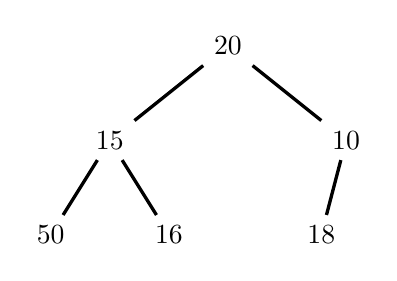
\begin{tikzpicture}[very thick,
  level distance=1.2cm,
  level 1/.style={sibling distance=3cm},
  level 2/.style={sibling distance=1.5cm}]
  \node {20}
    child {node {15}
      child {node {50}}
      child {node {16}}
    }
    child {node {10}
      child {node[left] {18}}
    };
\end{tikzpicture}
\end{center}

\textbf{Step 1 - sift-down at index 2 (value 10)} \\
Swap: 10 $\rightarrow$ 18
\textbf{Step 2 - sift-down at index 1 (value 15)} \\
Swap: 15 $\rightarrow$ 50
\textbf{Step 3 - sift-down at index 0 (value 20)} \\
Swap: 20 $\rightarrow$ 50

\textbf{Final heap:}

\begin{center}
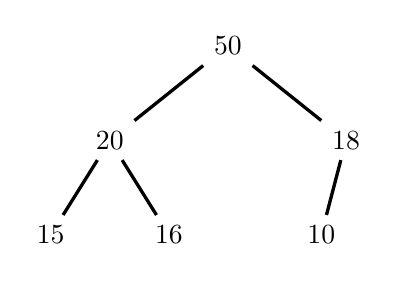
\begin{tikzpicture}[
  very thick,
  level distance=1.2cm,
  level 1/.style={sibling distance=3cm},
  level 2/.style={sibling distance=1.5cm}]
  \node {50}
    child {node {20}
      child {node {15}}
      child {node {16}}
    }
    child {node {18}
      child {node[left] {10}}
    };
\end{tikzpicture}
\end{center}

\subsubsection{Hashing}
\textbf{3. Insert the following keys using linear probing to a hash table of size 6: [20, 15, 10, 50, 16, 18]. The load factor in this case is 1. Show the completed hash table.}

\textbf{Solution:}

\begin{center}
\begin{tabular}{|c|c|}
\hline
\textbf{Index} & \textbf{Key} \\
\hline
0 & 16 \\
\hline
1 & 18 \\
\hline
2 & 20 \\
\hline
3 & 15 \\
\hline
4 & 10 \\
\hline
5 & 50 \\
\hline
\end{tabular}
\end{center}




% \documentclass{article}
% \usepackage{amsmath,amsfonts}
% \usepackage{tikz}
% \usepackage{geometry}
% \geometry{margin=1in}
% \title{Solutions: Class Test \#3 [2024-25] \\
% \large Data Structures, Algorithms and Databases}
% \author{}
% \date{}

\subsection{Question 1: Entity-Relationship Modelling}

A database system is needed customer account management of a stock brokerage house.

The requirements are as follows:

The stock brokerage house has customers that maintain investment accounts with them. Each account holds a certain number of ``securities" (shares, bonds etc.) and a cash balance. The securities are issued by authorised financial institutions and are identified by an ISIN (International Securities Identification Number). In addition, securities are also traded on a stock exchange which identifies them with a short ``trading symbol". For example, ``BARC" is the symbol assigned Barclays shares on the London Stock Exchange, while their ISIN is ``GB0031348658". The trading symbols are subject to change while the ISINs are fixed.

Securities are traded upon request from the customers. A trade may be for either buying or selling a specified number of securities. The database should record each trade transaction, the date and time when it took place, the price, quantity of securities bought or sold, and the commission charged.

Securities provide periodic income in the form of interest or dividends, which get credited to the account that holds the securities. Each income transaction should also be recorded along with the issuing institution and date.

\subsection*{(a) Entity-Relationship Model with Design Decisions and Multiplicities}

The main entities are:
\begin{itemize}
  \item \texttt{customer}
  \item \texttt{account}
  \item \texttt{security}
  \item \texttt{trade}
  \item \texttt{income}
\end{itemize}

Optionally, we may also treat an institution as an entity. We may define subclass entities for buying and selling trade transactions.

\bigskip

\noindent \textbf{TikZ ER Diagram:}
\begin{center}
\begin{tikzpicture}[node distance=2cm, every node/.style={draw, font=\small}]
  \node (customer) {Customer};
  \node[below of=customer] (account) {Account};
  \node[below of=account] (trade) {Trade};
  \node[right of=account, xshift=4cm] (security) {Security};
  \node[below of=security] (income) {Income};
  \node[above right=1.5cm and 2cm of security] (institution) {Institution};

  \draw (customer) -- node[left]{1..n} (account);
  \draw (account) -- node[below left]{1..n} (trade);
  \draw (account) -- node[below]{0..n} (security);
  \draw (trade) -- node[below]{1} (security);
  \draw (account) -- node[below right]{0..n} (income);
  \draw (income) -- node[right]{1} (security);
  \draw (security) -- node[right]{1} (institution);
\end{tikzpicture}
\end{center}

Comments: Almost all the relationships use (1,1) for unique and (0,n) for ``many". For example, an account is owned by a single customer. So it participates in the ``owns" relationship exactly once. A customer may own many accounts.

It is acceptable to use (1,n) for the ``many" multiplicity, but not ideal because it can cause problems in abnormal situations. For example, if the only account of a customer is to be deleted, then the customer would end up with fewer than 1 account.

The many-to-many relationship between account and security is crucial.

It is possible to treat income as a relationship, between account, security and institution. It results in the same tables as this design. \texttt{trade} can also be treated as a relationship (perhaps as two separate relations for ``buys" and ``sells").

It is okay to omit the institution entirely as an entity, because nothing is needed about it other than its name.

\subsection*{(b) Logical Design with Relational Schemas}

\begin{verbatim}
customer(custid, lastname, firstname, address, email)
account(accid, custid, cash)
security(ISIN, symbol, name, institution)
institution(name, address)
acc_security(accid, security)
trade(tradeid, accid, security, buy_or_sell, qty, date, time, price, commission)
income(accid, security, date, type, amount)
\end{verbatim}

Comments:

We need a table for every entity, except institution, which can possibly be treated as an attribute.

Only one relationship, \texttt{holds}, needs a table, here written as \texttt{acc\_security}.

All other relationships can be absorbed into entities.
\begin{itemize}
  \item \texttt{owns} absorbed into \texttt{account}.
  \item \texttt{orders} and \texttt{for} absorbed into \texttt{trade}.
  \item \texttt{issued by} absorbed into \texttt{security}.
  \item \texttt{issued by} for \texttt{income} also absorbed into \texttt{income}.
\end{itemize}

Note that we do not store the quantity of security held in the account, because it would be redundant: it can be calculated by looking through the trades for that security. If a student stores the quantity as an attribute, make a comment on it, but do not deduct points.

We keep a single table for \texttt{trade}, subsuming both the subclasses into it. It is also possible to have two separate tables for purchases and sales, or three tables: \texttt{trade}, \texttt{purchases} and \texttt{sales}.

\subsection*{(c) SQL \texttt{CREATE TABLE} Statements}

\begin{verbatim}
create table customer(
  custid INTEGER not null unique primary key,
  lastname VARCHAR(15) not null,
  firstname VARCHAR(15) not null,
  address VARCHAR(100) not null,
  phone DECIMAL(15) not null,
  email VARCHAR(100) not null
);

create table account(
  accid INTEGER not null unique primary key,
  custid INTEGER not null REFERENCES customer(custid),
  cash DECIMAL(10,2) not null
);

create table security(
  ISIN VARCHAR(10) not null unique,
  symbol VARCHAR(4) not null unique,
  name VARCHAR(100) not null,
  institution VARCHAR(20) not null REFERENCES institution(name)
);

create table institution(
  name VARCHAR(20) not null unique PRIMARY KEY,
  address VARCHAR(100) not null
);

create table acc_security(
  accid INTEGER not null REFERENCES account(accid) ON DELETE CASCADE,
  security VARCHAR(10) not null REFERENCES security(ISIN),
  primary key (accid, ISIN)
);

create table trade(
  tradeid INTEGER not null PRIMARY KEY GENERATED ALWAYS BY IDENTITY,
  accid INTEGER not null REFERENCES account(accid) ON DELETE CASCADE,
  security VARCHAR(10) not null REFERENCES security(ISIN),
  buy_or_sell SMALLINT,
  qty INTEGER not null,
  date DATE not null,
  time TIME not null,
  price DECIMAL(10,2) not null,
  commission DECIMAL(4,2) not null
);

create table income(
  accid INTEGER not null REFERENCES account(accid) ON DELETE CASCADE,
  security VARCHAR(10) not null REFERENCES security(ISIN),
  date DATE not null,
  type CHAR not null,
  amount DECIMAL(10,2) not null
);
\end{verbatim}

Most of the \texttt{ON DELETE} constraints are not written in the solution above, which means that the default of \texttt{ON DELETE NO ACTION} would be used.

It is possible to say \texttt{ON DELETE SET NULL} for the references to clients and workers, but then the \texttt{not null} constraint should be deleted.

\texttt{ON DELETE CASCADE} is used for references to accounts, since when an account is deleted, all its transactions have no further relevance.

\textbf{Note:} When an account is to be closed, all the securities held in it would need to be liquidated and the final cash balance would need to be paid out. Only after all this is done should the account be deleted, at which time its trades etc. can be deleted automatically.

On the other hand, we are prohibiting a customer from being deleted when their account still exists. The account should be closed and deleted before the customer can be deleted.
